\chapter{Propuesta de solución}
La propuesta de solución que se detalla a continuación constituye la respuesta técnica a la problemática de integridad académica analizada en los capítulos precedentes. A partir del planteamiento del problema y su justificación, se ha identificado la necesidad crítica de contar con herramientas de validación capaces de enfrentar los desafíos actuales en la enseñanza de la programación, especialmente ante el auge de soluciones generadas de forma automatizada.

Considerando las limitaciones detectadas en el estudio del estado del arte, donde los métodos de cotejo tradicionales han perdido efectividad frente a las nuevas técnicas de paráfrasis de código, y fundamentándose en los conceptos de análisis semántico y estilométrico explorados en el marco teórico, se propone el desarrollo de Graphito.

Graphito se define como un sistema de comparación de código diseñado para actuar como una herramienta de apoyo a la evaluación docente en cursos introductorios de programación en C/C++. La solución se basa en el análisis semántico del código fuente, lo que permite evaluar la similitud lógica entre programas y detectar posibles patrones de generación mediante inteligencia artificial, con el fin de optimizar el proceso de evaluación y fortalecer la integridad académica en el entorno educativo.

De esta manera, el sistema se constituye como un comparador integral que no solo realiza un contraste superficial, sino que coteja la estructura funcional y la identidad de las entregas frente a soluciones de referencia, proporcionando métricas objetivas que refuerzan el proceso de enseñanza-aprendizaje. En las secciones siguientes se describe la estructura operativa de la solución, iniciando con la representación esquemática de sus componentes funcionales y el flujo de procesamiento de la información, tal como se ilustra en el siguiente diagrama de bloques.

\section{Estructura Funcional del Sistema}

Para materializar el proceso de cotejo avanzado, Graphito se articula a través de una arquitectura de bloques funcionales que procesan la información de manera secuencial y paralela. En la Figura~\ref{fig:diagrama_bloques} se presenta el diagrama de bloques que describe el flujo de los datos, desde la ingesta del código fuente hasta la generación del reporte de similitud.

\begin{figure}[H] % [H] fuerza a que la imagen se quede justo aquí
    \centering
    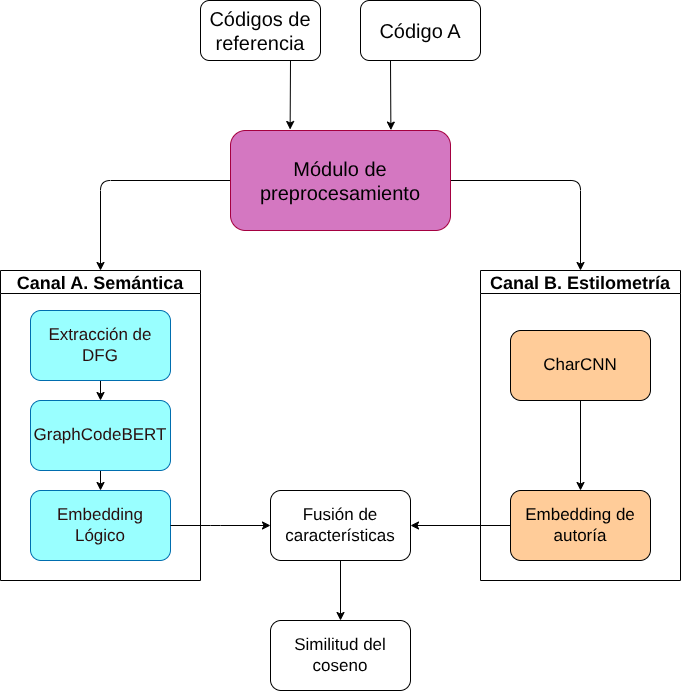
\includegraphics[width=0.8\textwidth]{figuras/diagrama_bloques.png} % Ajusta el ancho al 90% de la página
    \caption{Diagrama de bloques funcional del sistema de comparación Graphito.}
    \label{fig:diagrama_bloques} % Esta es la "etiqueta" para referenciarlo
\end{figure}

A continuación, se describen los componentes core que integran la solución:


%%%%%%%%%%%%%%%%%%%%%%%%%%%%%%%%%%%%%%%%%%%%%%%%%%%%%%%%%%%%%%%%%%%%%%%%%%%%%%%%%%%%
\subsection{Entrada de datos y fuentes de referencia}

El proceso de comparación comienza con la recepción de dos flujos de información fundamentales:

\begin{itemize}
    \item \textbf{Entrega del Alumno:} Archivos en formato fuente (.c o .cpp) que contienen la resolución propuesta por el estudiante a un problema en específico. El sistema está diseñado para procesar código basado en los estándares C11 y C++17, enfocandose en temas introductorios a la programacion como fundamentos y algoritmos y estructuras de datos. 
    
    \item \textbf{Códigos de Referencia:} Representan el conjunto de comparación, representando una o múltiples soluciones correctas al problema planteado. Este repositorio incluye la solución ideal proporcionada por el docente y, de manera complementaria, un conjunto de variantes funcionalmente equivalentes obtenidas mediante modelos de lenguaje (LLM). Esta diversidad de referencias permite que el sistema realice un cotejo robusto contra múltiples implementaciones lógicas de un mismo problema.
\end{itemize}

%%%%%%%%%%%%%%%%%%%%%%%%%%%%%%%%%%%%%%%%%%%%%%%%%%%%%%%%%%%%%%%%%%%%%%%%%%%%%%%%%%%%%%

\subsection{Módulo de Preprocesamiento y Normalización}

Una vez ingresados los archivos, el \textbf{Módulo de Preprocesamiento} genera dos representaciones distintas a partir de un mismo archivo fuente para satisfacer los requerimientos de cada canal de análisis:

\begin{enumerate}
    \item \textbf{Representación Normalizada (Canal A):} Se realiza una limpieza profunda de ambos conjuntos de código, eliminando comentarios, metadatos y espacios en blanco redundantes. Asimismo, se aplican técnicas de normalización de identificadores. Este proceso garantiza que el análisis semántico se enfoque exclusivamente en la topología del flujo de datos y la lógica algorítmica, ignorando cambios estéticos o de nomenclatura.
    \item \textbf{Representación Estructural/Raw (Canal B):} Se aplica únicamente a la solución del alumno. El sistema preserva elementos como la indentación, el uso de comentarios, la acentuación y caracteres especiales. Esta decisión técnica es clave para la detección de patrones de generación por IA, ya que permite identificar la "perfección" gramatical y hábitos de formato que constituyen la "huella digital" del autor o del modelo generativo utilizado.
\end{enumerate}

Una vez terminado ambos procesos, el flujo sigue hacia los canales de comparación semántica y analisis estilometríco. 

%%%%%%%%%%%%%%%%%%%%%%%%%%%%%%%%%%%%%%%%%%%%%%%%%%%%%%%%%%%%%%%%%%%
% 7.2 CANAL A: COMPARACIÓN SEMÁNTICA
%%%%%%%%%%%%%%%%%%%%%%%%%%%%%%%%%%%%%%%%%%%%%%%%%%%%%%%%%%%%%%%%%%%
\subsection{Canal A: Comparación Semántica}

Este canal constituye el componente principal para la identificación de equivalencias lógicas profundas, permitiendo detectar clones de código que comparten el mismo propósito algorítmico a pesar de presentar variaciones sintácticas. 

\subsubsection{Justificación y Selección del Modelo}

La selección de \textbf{GraphCodeBERT} \cite{Guo2021GraphCodeBERT} como motor de análisis semántico responde a la necesidad de superar las limitaciones de los modelos puramente secuenciales (como CodeBERT o Transformers estándar). La decisión se fundamenta en los siguientes pilares técnicos:

\begin{itemize}
    \item \textbf{Integración Estructural:} A diferencia de otros modelos que tratan el código como una simple secuencia de texto, GraphCodeBERT integra información estructural mediante el uso de grafos de flujo de datos (DFG). Esto permite que el mecanismo de atención se centre en las conexiones que tienen sentido semántico real.
    \item \textbf{Resistencia a la Ofuscación:} Debido a que el modelo captura la relación entre variables (\textit{def-use chains}), es altamente efectivo detectando similitudes incluso cuando el código ha sido alterado mediante cambios de nombres de variables, reordenamiento de sentencias o cambios en las estructuras de control.
    \item \textbf{Especialización Funcional:} Como se detalla en el marco teórico, este modelo se especializa en el comportamiento lógico del programa. Si bien tiende a ignorar rasgos superficiales como el estilo, esta característica se alinea perfectamente con la arquitectura bimodal de Graphito, delegando la responsabilidad del análisis de estilo al Canal B (CharCNN).
\end{itemize}



\subsubsection{Extracción de Grafo de Flujo de Datos (DFG)}

Un Grafo de Flujo de Datos (DFG) es una representación dirigida que captura las dependencias funcionales entre las variables de un programa mediante la identificación de sus relaciones de definición y uso (\textit{def-use chains}). De acuerdo con la metodología propuesta por Guo et al. \cite{Guo2021GraphCodeBERT}, los pasos para obtener esta representación son:

\begin{enumerate}
    \item \textbf{Generación del AST (Análisis sintáctico):} El código fuente se procesa para construir su Árbol de Sintaxis Abstracta (AST), obteniendo la jerarquía gramatical del programa.
    \item \textbf{Identificación de la secuencia de variables:} Se analizan los nodos terminales (hojas) del AST para extraer todas las variables presentes, preservando su orden de aparición.
    \item \textbf{Definición de los nodos del grafo:} Cada ocurrencia de una variable se establece como un nodo individual dentro del grafo.
    \item \textbf{Construcción de las aristas (Dependencias de valor):} Se trazan enlaces dirigidos entre nodos $v_i$ y $v_j$ si el valor de la variable $v_j$ depende directamente de la definición o valor previo de $v_i$.
\end{enumerate}

\subsubsection{Procesamiento en GraphCodeBERT}

Una vez construido el DFG, la secuencia de \textit{tokens} del código y la estructura del grafo se integran en el modelo. La arquitectura utiliza tareas de entrenamiento como la predicción de relaciones entre nodos, lo que favorece el aprendizaje de representaciones mucho más estructuradas y fieles al comportamiento funcional del software.

\subsubsection{Embedding Lógico}

El resultado final de este canal es un \textbf{Embedding Semántico}: un vector denso de alta dimensionalidad que actúa como una firma lógica del programa. Este vector permite realizar comparaciones de proximidad matemática, identificando si dos soluciones son funcionalmente iguales sin importar la forma en que fueron escritas.
%%%%%%%%%%%%%%%%%%%%%%%%%%%%%%%%%%%%%%%%%%%%%%%%%%%%%%%%%%%%%%%%%%%%%%%%%%%%%%%%%%%%%%%%%%%%%%%%%%%%

\subsection{Canal B: Comparación Estilométrica}

Mientras que el Canal A se encarga de la profundidad lógica, el Canal B se enfoca en la superficie del código. Para esta tarea, se seleccionó el modelo \textbf{CharCNN} \cite{Zhang2015CharCNN} sobre otras arquitecturas de procesamiento de lenguaje natural más complejas por una razón de eficiencia y diseño: al contar ya con un modelo de alta capacidad para el análisis semántico, no es necesario un segundo modelo que intente comprender la sintaxis global. En su lugar, se requiere un extractor de rasgos que sea capaz de ``ver'' el código como una señal visual.

\subsubsection{Justificación y Selección del Modelo}

La elección de una Red Neuronal Convolucional a nivel de caracteres (CharCNN) responde a su capacidad innata para actuar como un escáner de patrones locales. Dado que las CNN son especialistas en visión computacional, al aplicarlas al código fuente ``en bruto'' (\textit{raw code}), el modelo puede identificar automáticamente rasgos que para otros sistemas serían invisibles:

\begin{itemize}
    \item \textbf{Estilo como Señal Visual:} El modelo interpreta la indentación, el uso de espacios y la disposición de caracteres especiales como texturas visuales, permitiendo aprender el estilo del autor sin necesidad de conocer la gramática del lenguaje C++.
    \item \textbf{Detección de Hiper-perfección:} Mientras que un estudiante suele presentar una escritura heterogénea y con errores humanos de formato, los modelos de lenguaje (LLM) generan código con una estructura y puntuación gramaticalmente perfecta en los comentarios. CharCNN es ideal para detectar esta ``perfección'' sintética que delata el uso de IA.
    \item \textbf{Eficiencia Computacional:} Al operar localmente sobre secuencias de caracteres, el modelo aporta una capa de seguridad adicional sin incrementar drásticamente la carga computacional del sistema \textit{backend}.
\end{itemize}



\subsubsection{Análisis de Autoría mediante CharCNN}

El procedimiento estructurado para transformar el código fuente en un identificador de estilo se detalla a continuación:

\begin{enumerate}
    \item \textbf{Preservación de Código Raw:} Se utiliza la versión del código que conserva comentarios, sangrías y acentuación, elementos que suelen ser eliminados en análisis tradicionales pero que son críticos para la detección de la firma del autor.
    \item \textbf{Mapeo de Caracteres:} El texto se transforma en una secuencia de índices numéricos basados en un alfabeto predefinido, permitiendo que la red procese el código como una señal discreta y medible.
    \item \textbf{Extracción Convolucional de Rasgos:} Se aplican filtros convolucionales de distintos tamaños para detectar ``n-gramas'' de caracteres. Esto permite identificar hábitos microscópicos, como la preferencia por ciertos operadores o la pulcritud en la redacción de comentarios.
    \item \textbf{Reducción de Dimensionalidad (Pooling):} Se seleccionan las características más relevantes detectadas por los filtros, consolidando los rasgos estilísticos más distintivos de la muestra analizada en una representación compacta.
\end{enumerate}

\subsubsection{Generación de Embedding de Autoría}

Una vez procesada la información por las capas convolucionales, el sistema genera un \textbf{Embedding de Autoría}. Este vector denso representa la ``huella digital'' del emisor, capturando las sutilezas que diferencian la redacción manual de un estudiante de la generación estandarizada de un LLM.

Este embedding es fundamental para Graphito, ya que permite alertar al docente cuando la lógica de un programa coincide con la de una referencia, pero el estilo de escritura sugiere una procedencia no humana. En términos prácticos, el Canal B actúa como el detector de anomalías que complementa el juicio semántico del Canal A.

%%%%%%%%%%%%%%%%%%%%%%%%%%%%%%%%%%%%%%%%%%%%%%%%%%%%%%%%%%%%%%%%%%%%%%%%%%%%%%%%%%%%%%%%%%%%%%%%%%%%%
\subsection{Fusión de Características}

La fusión de características \cite{MartinezGil2026Improving} representa el proceso de integración donde las salidas de los canales semántico y estilométrico convergen para formar una representación única y bimodal de la entrega. 

Este bloque técnico es fundamental para el sistema Graphito, ya que permite consolidar dos dimensiones de análisis distintas en un solo espacio vectorial:

\begin{itemize}
    \item \textbf{Mecanismo de Integración:} El sistema toma el \textbf{Embedding Semántico} (que encapsula la lógica extraída por GraphCodeBERT) y el \textbf{Embedding de Autoría} (que contiene los rasgos estructurales detectados por CharCNN) y los combina mediante una operación de concatenación. En el caso de las soluciones de referencia, se aplica un acolchado de ceros (\textit{zero-padding}) en las dimensiones correspondientes al canal estilométrico, garantizando la homogeneidad dimensional necesaria para el cálculo de similitud.
    
    \item \textbf{Generación de la Firma Bimodal:} El resultado de esta fusión es un vector de características unificado que actúa como una "firma digital" del código. Esta firma no solo describe qué funciones realiza el programa, sino que también preserva los hábitos de escritura y formato del emisor.
\end{itemize}

Al integrar ambos tipos de información, la fusión permite que el sistema tenga una comprensión profunda del código, facilitando la detección de anomalías donde la lógica del programa es correcta pero el estilo de redacción es inconsistente con el perfil esperado, lo que constituye un indicio clave de asistencia por inteligencia artificial.

%%%%%%%%%%%%%%%%%%%%%%%%%%%%%%%%%%%%%%%%%%%%%%%%%%%%%%%%%%%%%%%%%%%
% 7.5 SIMILITUD DEL COSENO
%%%%%%%%%%%%%%%%%%%%%%%%%%%%%%%%%%%%%%%%%%%%%%%%%%%%%%%%%%%%%%%%%%%
\subsection{Similitud del Coseno}

La Similitud del Coseno es una métrica matemática que mide el coseno del ángulo entre dos vectores en un espacio multidimensional. A diferencia de otras métricas de distancia, esta no se ve afectada por la magnitud de los vectores (en este caso, la longitud del código), sino por su orientación, lo que la hace ideal para comparar la esencia de dos fragmentos de software.

La similitud entre la entrega del alumno ($A$) y el código de referencia ($R$) se calcula mediante la siguiente fórmula:

\begin{equation}
\text{sim}(A, R) = \frac{A \cdot R}{\|A\| \|R\|} = \frac{\sum_{i=1}^{n} A_i R_i}{\sqrt{\sum_{i=1}^{n} A_i^2} \sqrt{\sum_{i=1}^{n} R_i^2}}
\label{eq:coseno}
\end{equation}

El resultado de esta operación oscila en el intervalo $[0, 1]$, donde $1$ representa una coincidencia total de orientación y $0$ una independencia absoluta entre los vectores.

\subsubsection{Importancia de la Métrica en la Fusión de Características}

El uso de esta métrica es fundamental en Graphito debido a la naturaleza asimétrica de la fusión de características. Al combinar el análisis semántico (lógica) y el estilométrico (IA), la similitud del coseno actúa no solo como un comparador, sino como un regulador de integridad académica.



La relevancia de utilizar este enfoque bimodal radica en los siguientes puntos:

\begin{itemize}
    \item \textbf{Efecto de la Carga Estilística:} Para el sistema, el código del profesor es el "estándar de verdad", por lo que su vector se proyecta con una componente de estilo neutra. Si un alumno entrega un código con lógica perfecta pero generado por una IA, su vector adquirirá una "carga extra" en la dimensión del estilo.
    \item \textbf{Desviación del Vector:} Aunque el código del alumno sea funcionalmente idéntico al del profesor, la presencia de rasgos sintéticos (detectados por el Canal B) hace que el vector del alumno se "desvíe" o rote respecto al del profesor. Esta desviación incrementa el ángulo entre ambos, reduciendo automáticamente el valor de la similitud final.
    \item \textbf{Penalización Intrínseca:} Gracias a la propiedad del denominador en la fórmula (la norma del vector $\|A\|$), cualquier rastro de IA detectado incrementa la magnitud del vector del alumno sin aportar al numerador. Esto castiga la calificación de similitud de manera proporcional a la "perfección" sintética detectada, permitiendo diferenciar entre un alumno que programó honestamente y uno que utilizó asistencia externa.
\end{itemize}

En conclusión, la Similitud del Coseno permite que Graphito entregue un veredicto más justo y profundo. No se limita a decir si el programa "funciona igual", sino que evalúa si la forma en que fue construido se alinea con el estándar humano de referencia, convirtiéndola en una métrica esencial para combatir el plagio moderno potenciado por inteligencia artificial.


\section{Conclusión}

La propuesta de solución presentada en este capítulo, denominada \textbf{Graphito}, se aleja de los enfoques de comparación de texto tradicionales para adoptar una arquitectura bimodal basada en aprendizaje profundo. A través de la integración del análisis semántico (Canal A) y el análisis estilométrico (Canal B), el sistema es capaz de evaluar el código fuente no solo por lo que hace, sino por la identidad de su escritura.

La principal fortaleza de esta propuesta reside en su capacidad de autorregulación mediante la similitud del cosenos asimétrica. Al tratar la lógica como el eje central y el estilo como un factor de penalización, Graphito ofrece una métrica de integridad académica robusta frente a las técnicas modernas de ofuscación y la generación sintética por modelos de lenguaje. 

Con la definición funcional de estos bloques y la fundamentación de sus componentes core, queda establecida la base teórica y metodológica de la solución. En el siguiente capítulo, se procederá con el Anal   , donde se detallará la arquitectura de software, la persistencia de datos y los diagramas de interacción necesarios para la implementación física de esta propuesta.